\documentclass[aspectratio=169]{beamer}
\usetheme{Bruno}
\usepackage{amsmath}
\usepackage{amssymb}
\usepackage{siunitx}
\usepackage{float}
\usepackage{tikz}
\def\checkmark{\tikz\fill[scale=0.4](0,.35) -- (.25,0) -- (1,.7) -- (.25,.15) -- cycle;} 
\usepackage{url}
\usepackage[siunitx,american,RPvoltages]{circuitikz}
\ctikzset{capacitors/scale=0.7}
\ctikzset{diodes/scale=0.7}
\usepackage{tabularx}
\newcolumntype{C}{>{\centering\arraybackslash}X}
\renewcommand\tabularxcolumn[1]{m{#1}}% for vertical centering text in X column
\usepackage{tabu}
\usepackage[spanish,es-tabla,activeacute]{babel}
\usepackage{babelbib}
\usepackage{booktabs}
\usepackage{pgfplots}
\usepackage{hyperref}
\hypersetup{colorlinks = true,
            linkcolor = black,
            urlcolor  = blue,
            citecolor = blue,
            anchorcolor = blue}
\usepgfplotslibrary{units, fillbetween} 
\pgfplotsset{compat=1.16}
\usepackage{bm}
\usetikzlibrary{arrows, arrows.meta, shapes, 3d, perspective, positioning,mindmap,trees,backgrounds}
\renewcommand{\sin}{\sen} %change from sin to sen
\usepackage{bohr}
\setbohr{distribution-method = quantum,insert-missing = true}
\usepackage{elements}
\usepackage{verbatim}
\usepackage[edges]{forest}
\usepackage{etoolbox}
\usepackage{schemata}
\usepackage{appendix}
\usepackage{listings}

\definecolor{color_mate}{RGB}{255,255,128}
\definecolor{color_plas}{RGB}{255,128,255}
\definecolor{color_text}{RGB}{128,255,255}
\definecolor{color_petr}{RGB}{255,192,192}
\definecolor{color_made}{RGB}{192,255,192}
\definecolor{color_meta}{RGB}{192,192,255}
\newcommand\diagram[2]{\schema{\schemabox{#1}}{\schemabox{#2}}}

\definecolor{codegreen}{rgb}{0,0.6,0}
\definecolor{codegray}{rgb}{0.5,0.5,0.5}
\definecolor{codepurple}{rgb}{0.58,0,0.82}
\definecolor{backcolour}{rgb}{0.95,0.95,0.92}

\lstdefinestyle{mystyle}{
    backgroundcolor=\color{backcolour},   
    commentstyle=\color{codegreen},
    keywordstyle=\color{magenta},
    numberstyle=\tiny\color{codegray},
    stringstyle=\color{codepurple},
    basicstyle=\ttfamily\footnotesize,
    breakatwhitespace=false,         
    breaklines=true,                 
    captionpos=b,                    
    keepspaces=true,                 
    numbers=left,                    
    numbersep=5pt,                  
    showspaces=false,                
    showstringspaces=false,
    showtabs=false,                  
    tabsize=2
}

\lstset{style=mystyle}
\title{Instrumentación I: \\ \emph{Medidas de}\\ \emph{presión   }}
\author{
    Juan J. Rojas, Hugo Sanchez Ortiz
}
\institute{Instituto Tecnológico de Costa Rica}
\date{\today}
\background{fig/background.jpg}
\begin{document}
\sisetup{unit-math-rm=\mathrm,math-rm=\mathrm} % change sinitx font
\sisetup{output-decimal-marker = {,}}
\maketitle

\newcommand{\blackandwhite}{white} %change this at the end

\begin{frame}{Definiciones}
    \begin{columns}[c, onlytextwidth]
        \begin{column}{0.50\textwidth}
            \begin{itemize}
                \item Es la magnitud de la fuerza que se aplica perpendicularmente a una superficie por unidad de área. 
                \item Presión diferencial: es la diferencia de presión entre dos puntos de medición
                \item Presión manométrica: es la presión medida respecto a la presión atmosférica. 
                \item Presión absoluta: es la presión medida respecto al vacío. 
            \end{itemize}
        \end{column}
        \begin{column}{0.45\textwidth}
            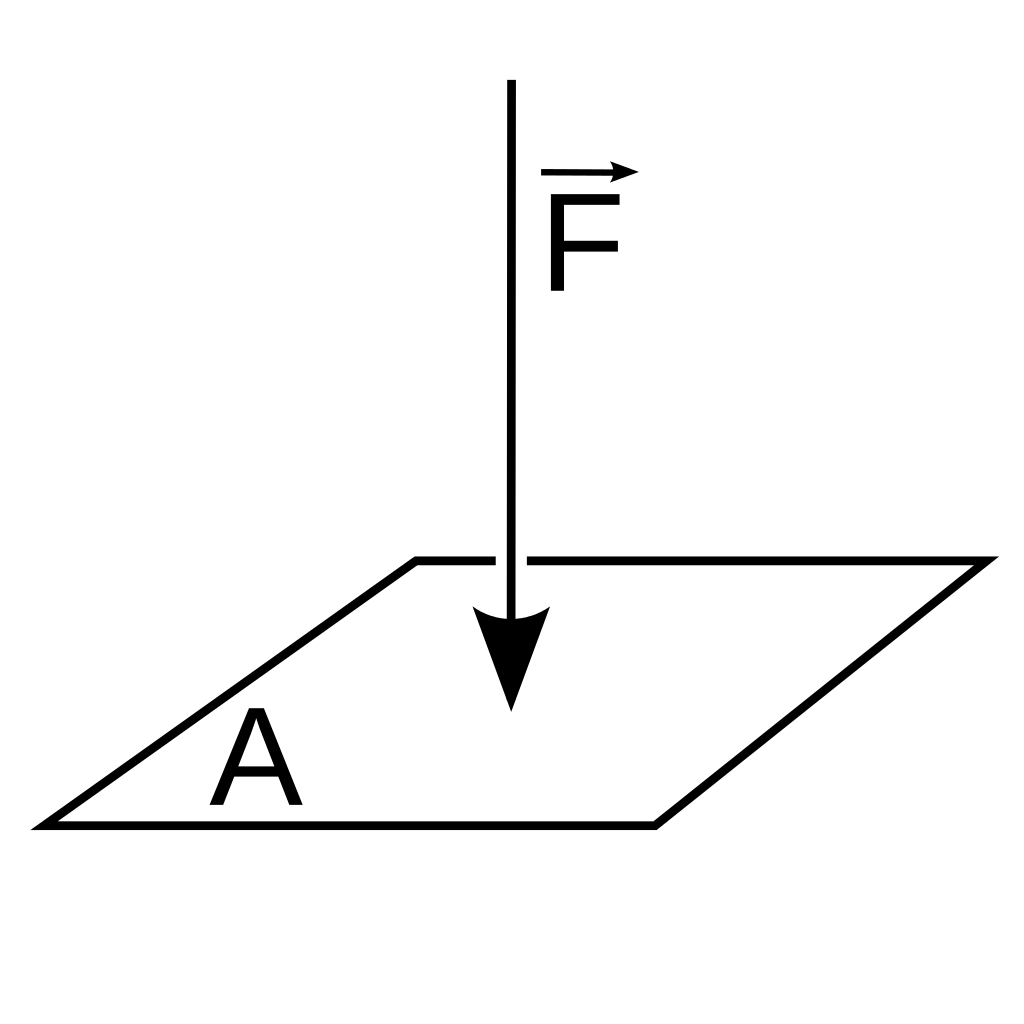
\includegraphics[width = 0.8\linewidth]{fig/pressure.png}
            
            \tiny{\href{https://commons.wikimedia.org/w/index.php?curid=25665611}{By Klaus-Dieter Keller - Own work, Public Domain}}
        \end{column}
    \end{columns}
\end{frame}

\begin{frame}{Unidades de medida} 
La unidad de medida de presión en el SI es el Pascal:
    \begin{equation*}
        \SI{1}{\pascal} = \dfrac{\si{\newton}}{\si{\meter\squared}} = \dfrac{\si{\kilogram}}{\si{\meter\cdot \second\squared}}
    \end{equation*}
Algunas equivalencias:
\begin{table}[c]
    \begin{tabular}{ccc}
        \toprule
        unidad & nombre & equivalencia en SI \\
        \midrule
        $1\mathrm{atm}$ & atmosfera & \SI{101325}{\pascal} \\
        $1\mathrm{bar}$ & bares & \SI{1e5}{\pascal}\\
        $1\mathrm{psi}$ & libras por pulgada cuadrada& \SI{6894,757}{\pascal} \\
        $1\mathrm{mm.c.d.a.}$ & mm de columna de agua & \SI{9.80665}{\pascal} \\
        $1\mathrm{mmHg}$ & mm de columna de mercurio & \SI{133322.4}{\pascal} \\
        \bottomrule
    \end{tabular}
    %\caption{Distintas unidades de presión}
    \label{tab:unid}
\end{table}
\end{frame}

\begin{frame}{Clases de Presión}
    \begin{columns}[c, onlytextwidth]
        \begin{column}{0.45\textwidth}
            \begin{itemize}
                \item \textbf{Absoluta}: Relación entre el cero absoluto de presión. 
                \item \textbf{Atmosférica}: Presión ejercida por la atmósfera terrestre. 
                \item \textbf{Relativa} diferencia entre absoluta y atmosférica. 
                \item \textbf{Diferencial}: Entre dos puntos.
                \item \textbf{Vacío} medida por debajo de la presión atmosférica.
            \end{itemize}
        \end{column}
        \begin{column}{0.50\textwidth}
            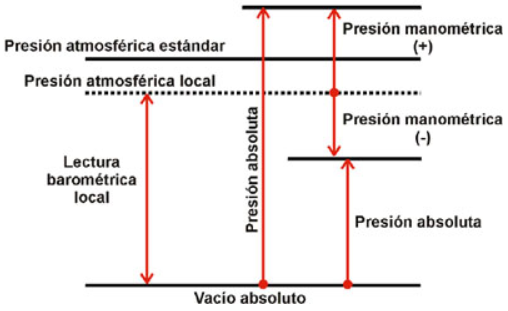
\includegraphics[width = 1.1\linewidth]{fig/Presion/Tipos.PNG}
            %\tiny{\href{https://commons.wikimedia.org/w/index.php?curid=25665611}{By Klaus-Dieter Keller - Own work, Public Domain}}
        \end{column}
    \end{columns}
\end{frame}

\begin{frame}{Instrumentos de presión}
    \begin{columns}[c, onlytextwidth]
        \begin{column}{0.45\textwidth}
        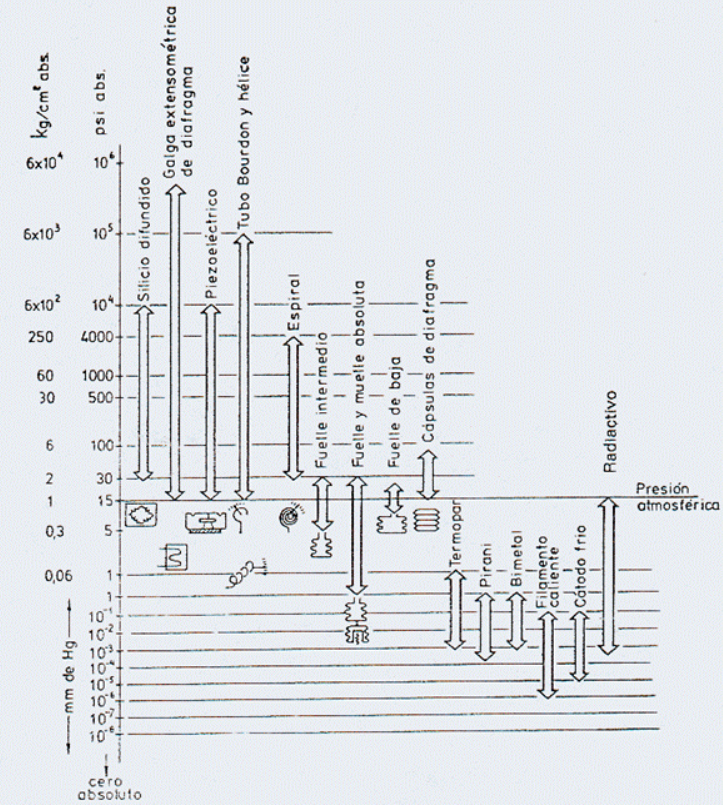
\includegraphics[width = 0.9 \linewidth]{fig/Presion/Instrumentos.PNG}
            
            \tiny{\cite{sole2005instrumentacion}}
            
        \end{column}
        \begin{column}{0.50\textwidth}
            \begin{itemize}
                \item Para cada una de las aplicaciones existen distintos tipos de sistemas de medición. 
                \item Por lo regular, los sistemas de medición por debajo y por encima de la presión atmosférica no son intercambiables.
            \end{itemize}
        \end{column}
    \end{columns}

            
\end{frame}

\begin{frame}{Métodos de medición de presión}
Para poder medir la presión esta se compara con una fuerza conocida o se mide su efecto sobre un elemento elástico.

\begin{enumerate}
    \item Columna de líquido + medición de nivel
    \item Elemento elástico
    \begin{enumerate}
        \item Tubo Bourdon + medición de desplazamiento
        % \begin{itemize}
        %     \item Potenciometro
        %     \item LVDT
        %     \item Inductivos
        % \end{itemize}
        \item Diafragma + medición de desplazamiento
        \begin{enumerate}
            \item Deformación central
            \item Deformación global
            \item Deformación local
        \end{enumerate}
    \end{enumerate}
    \item Elementos electromecánicos
    \item Elementos electrónicos de vacío
\end{enumerate}
\end{frame}


\begin{frame}{Medición por columna de líquido}
    \begin{columns}[c, onlytextwidth]
        \begin{column}{0.8\textwidth}
            \begin{itemize}
                \item Un manómetro de columna de líquido, como el tubo en U mostrado en la figura de la derecha, compara la presión medida con una presión de referencia y esto provoca una diferencia en el nivel de líquido. La diferencia de nivel esta dada por:
                \begin{equation*}
                    h = \dfrac{p-p_{ref}}{\rho g}
                \end{equation*}
                donde $\rho$ es la densidad del líquido y $g$ es la aceleración de la gravedad
                \item Se puede utilizar un sensor de nivel para obtener una señal eléctrica. 
            \end{itemize}
        \end{column}
        \begin{column}{0.2\textwidth}
            \centering
            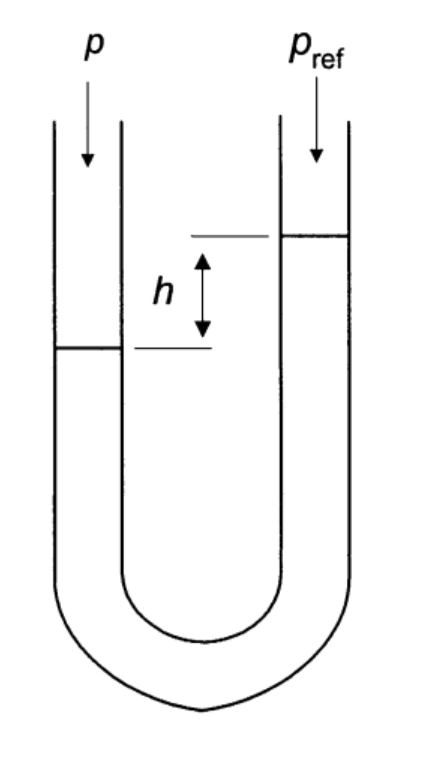
\includegraphics[width=3cm]{fig/Presion/columna.PNG}
             \\ \tiny{Tomado de \cite{pallas2012sensors}}
        \end{column}
    \end{columns}
\end{frame}

\begin{frame}{Manómetros mecánicos}
    \begin{columns}[c, onlytextwidth]
        \begin{column}{0.5\textwidth}
            \begin{itemize}
                \item Un tubo Bourdon es un tubo metálico aplanado que es doblado o retorcido y sellado en uno de sus extremos. 
                \item Cuando la presión ingresa por el extremo abierto el tubo tiende a enderezarse 
                \item El desplazamiento del extremo libre se puede medir con sensor de desplazamiento para obtener una señal eléctrica.
            \end{itemize}
        \end{column}
        \begin{column}{0.5\textwidth}
            \centering
            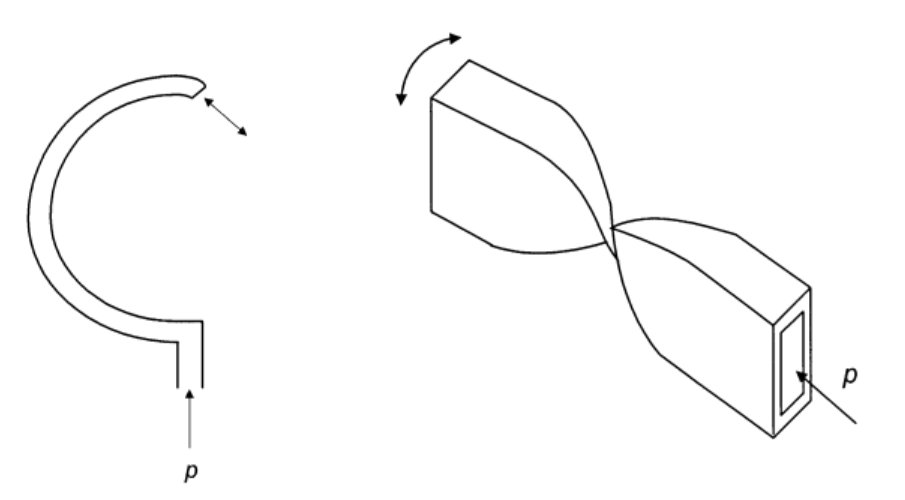
\includegraphics[width=7cm]{fig/Presion/bourdon.PNG}
             \\ \tiny{Tomado de \cite{pallas2012sensors}}
        \end{column}
    \end{columns}
\end{frame}

\begin{frame}{Membranas}
    \begin{columns}[c, onlytextwidth]
        \begin{column}{0.6\textwidth}
            \begin{itemize}
                \item Una membrana como la mostrada en la figura de la derecha se deforma debido a la diferencia entre la presión interna y externa.
                \item Se puede medir el desplazamiento del centro de la membrana, la deformación global o el esfuerzo local asociado a la deformación.
                \item Este tipo de membrana puede ser fabricada con procesos de microfabricación similares a los utilizados en semiconductores, en este caso se conoce como sensor MEMS.
            \end{itemize}
        \end{column}
        \begin{column}{0.4\textwidth}
            \centering
            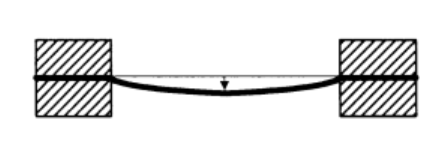
\includegraphics[width=5cm]{fig/Presion/membrana.PNG}
            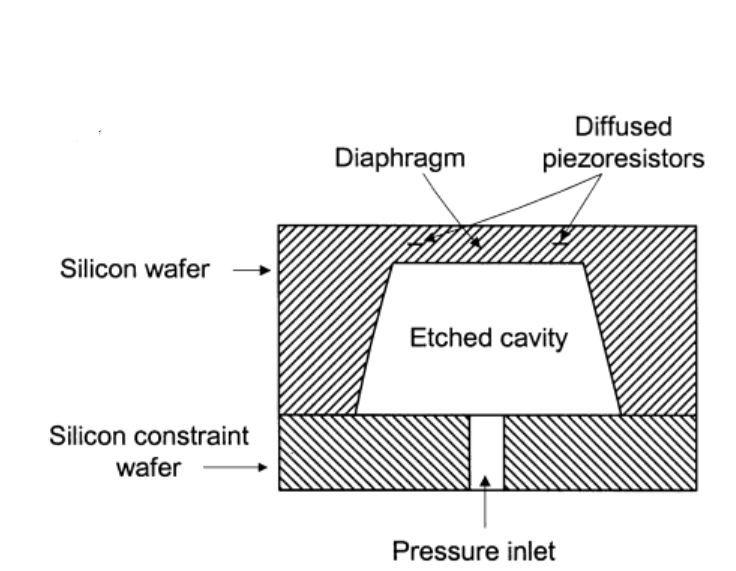
\includegraphics[width=5cm]{fig/Presion/memsmembrana.PNG}
             \\ \tiny{Tomado de \cite{pallas2012sensors}}
        \end{column}
    \end{columns}
\end{frame}

\begin{frame}{Piezoresistivos}
    \begin{columns}[c, onlytextwidth]
        \begin{column}{0.65\textwidth}
            \begin{itemize}
                \item Un piezoresistor es un elemento que cambia su resistencia según el esfuerzo al que sea sometido
                \item Un elemento piezoresistivo puede ser fabricado por difusión en una membrana microfabricada en silicio
                \item Los elementos se fabrican de forma que estén expuestos uno a esfuerzos longitudinales y el otro a esfuerzos trasversales de forma que sus contribuciones permitan una mayor sensibilidad. 
            \end{itemize}
        \end{column}
        \begin{column}{0.3\textwidth}
            \centering
            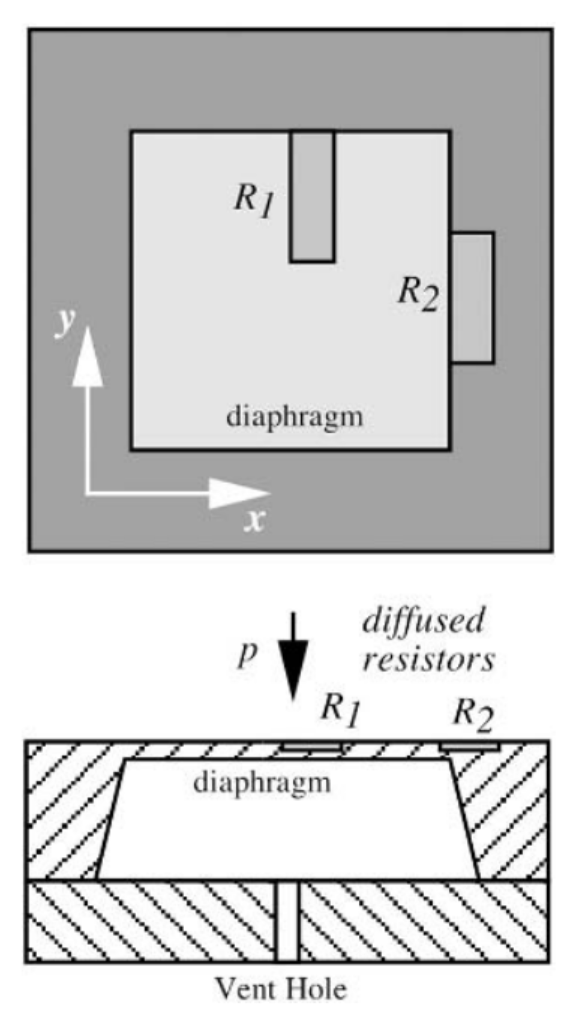
\includegraphics[width=3.5cm]{fig/Presion/piezores.PNG}
             \\ \tiny{Tomado de \cite{pallas2012sensors}}
        \end{column}
    \end{columns}
\end{frame}

\begin{frame}{Capacitivos}
    \begin{columns}[c, onlytextwidth]
        \begin{column}{0.5\textwidth}
            \begin{itemize}
                \item Dos placas de material conductivo forman un capacitor, si una de ella es una membrana se obtiene un capacitor variable. 
                \item Muy utilizados en micrófonos por su sensibilidad y buena respuesta a altas frecuencias, además de su resitencia a sobrepresiones. 
            \end{itemize}
        \end{column}
        \begin{column}{0.5\textwidth}
            \centering
            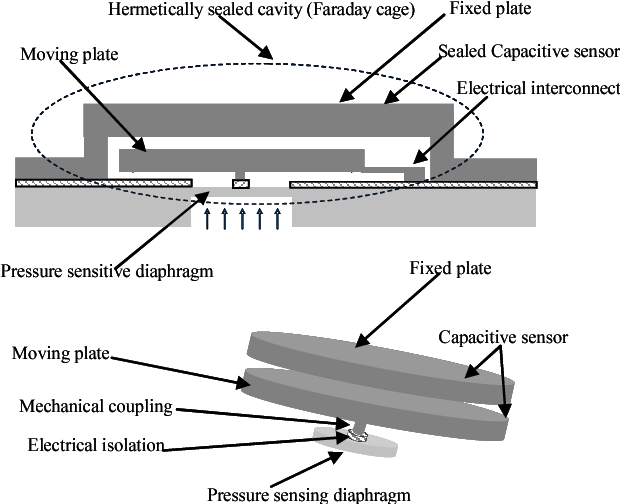
\includegraphics[width=6cm]{fig/Presion/memscapacitive.png}
             \\ \tiny{Tomado de \cite{pallas2012sensors}}
        \end{column}
    \end{columns}
\end{frame}

\begin{frame}{Capacitivos}
    Micrófono capacitivo usado en IPhone 4
    \begin{figure}
        \centering
        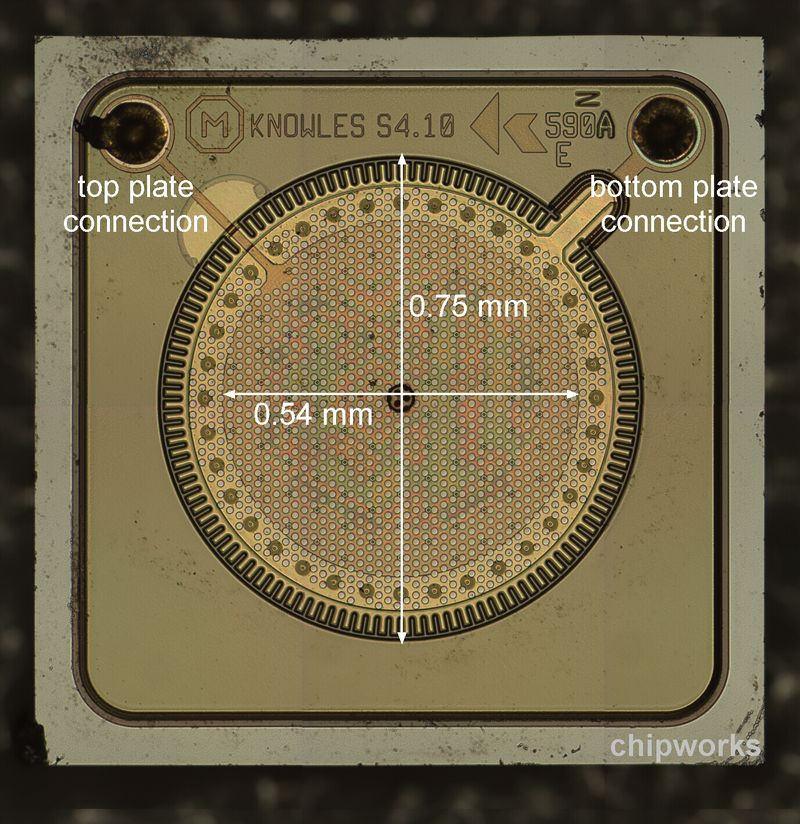
\includegraphics[width=4cm]{fig/Presion/memsmic.jpg}
        \tiny{Tomado de \href{https://www.memsjournal.com/2011/03/overview-of-mems-microphone-technologies-for-consumer-applications.html}{acá}}
    \end{figure}
\end{frame}

\begin{frame}{Magnéticos}
    \begin{columns}[c, onlytextwidth]
        \begin{column}{0.6\textwidth}
            \begin{itemize}
                \item Un sensor de presión de reluctancia variable es un transformador diferencial al que se le modula su reluctancia por medio de la deformación de un diafragma que cierra el circuito magnético. 
                \item La deformación produce cambio en la brecha de aire entre el núcleo en forma de E y el diafragma y de esta manera se obtiene un cambio en la reluctancia. 
                \item Este tipo de sensores es muy sensible a bajas presiones debido a que típicamente sus deflexiones no sobrepasan los $25$ a $\SI{30}{\micro\meter}$ 
            \end{itemize}
        \end{column}
        \begin{column}{0.4\textwidth}
            \centering
            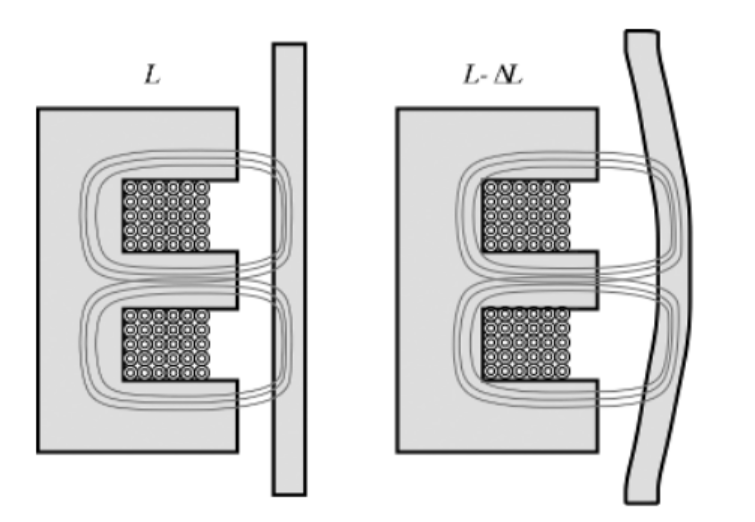
\includegraphics[width=6cm]{fig/Presion/VRP.PNG}
             \\ \tiny{Tomado de \cite{pallas2012sensors}}
        \end{column}
    \end{columns}
\end{frame}

\begin{frame}{Elementos Electromecánicos }
    \begin{columns}[c, onlytextwidth]
        \begin{column}{0.5\textwidth}
            \begin{itemize}
                \item Combinan un elemento mecánico, como los vistos anteriormente, con un transductor eléctrico. 
                \item Varios tipos:
             \begin{itemize}
                 \item Resistivos
                 \item Magnéticos
                 \item Capacitivos
                 \item Extensiométricos
                 \item Piezoeléctricos
             \end{itemize}
            \end{itemize}
        \end{column}
        \begin{column}{0.5\textwidth}
            \centering
            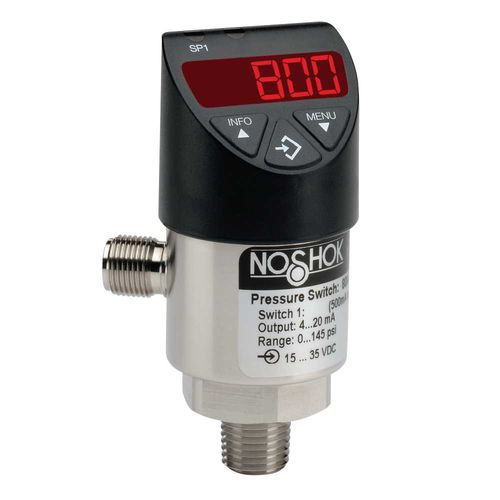
\includegraphics[width=6cm]{fig/Presion/EM_Sensor.jpg}
             \\ \tiny{\href{https://www.directindustry.com/prod/noshok/product-26191-462375.html}{Sensor Electromecánico de Presión}}
        \end{column}
    \end{columns}
\end{frame}

\begin{frame}{Elementos Electromecánicos }
 \begin{table}[]
 \footnotesize
    \centering
    \begin{tabular}{m{3.2cm} m{1.2cm} m{1.2cm} m{1.9cm} m{1.8cm} m{1.6cm}}
        \toprule
        \textbf{Tipo de Sensor} & \textbf{Margen [bar]} & \textbf{Exactitud [$\%$]} &\textbf{Estabilidad} & \textbf{Sobrecarga} & \textbf{Nivel de Señal} \\
        \midrule
        \textbf{Resistivo} & 2-6000 & 0.5 & Media a mala & 150 \% & 10 V\\
        \textbf{Magnético (Inductancia Variable)} & 0-0.1 & 0.5 & Mala & 150 \% & Variable\\
        \textbf{Magnético (Reluctancia Variable)} & 0-300 & 0.5 & Media & 150 \% & 0-5 V\\
        \textbf{Capacitivos} & 0-3000 & 0.5 & Media a buena & 150 \% & 0-5  V\\
        \textbf{Galgas Cementadas} & 0-3000 & 0.5 & Mala & 150 \% & 35 mV\\
        \textbf{Galgas sin Cementar} & 0-600 & 0.5 & Mala & 200 \% & 35 mV\\
        \textbf{Piezoeléctrico} & 0-600 & 1 & Mala & 200 \% & 600 mV/bar\\
        \bottomrule
    \end{tabular}
    \caption{Comparación entre distintos tipos de presión electromecánicos \cite{sole2005instrumentacion}}
    \label{tab:Comparacion}
\end{table}
\end{frame}

\begin{frame}{Elementos Electrónicos de Vacío}
    \begin{columns}[c, onlytextwidth]
    
     \begin{column}{0.5\textwidth}
            \centering
            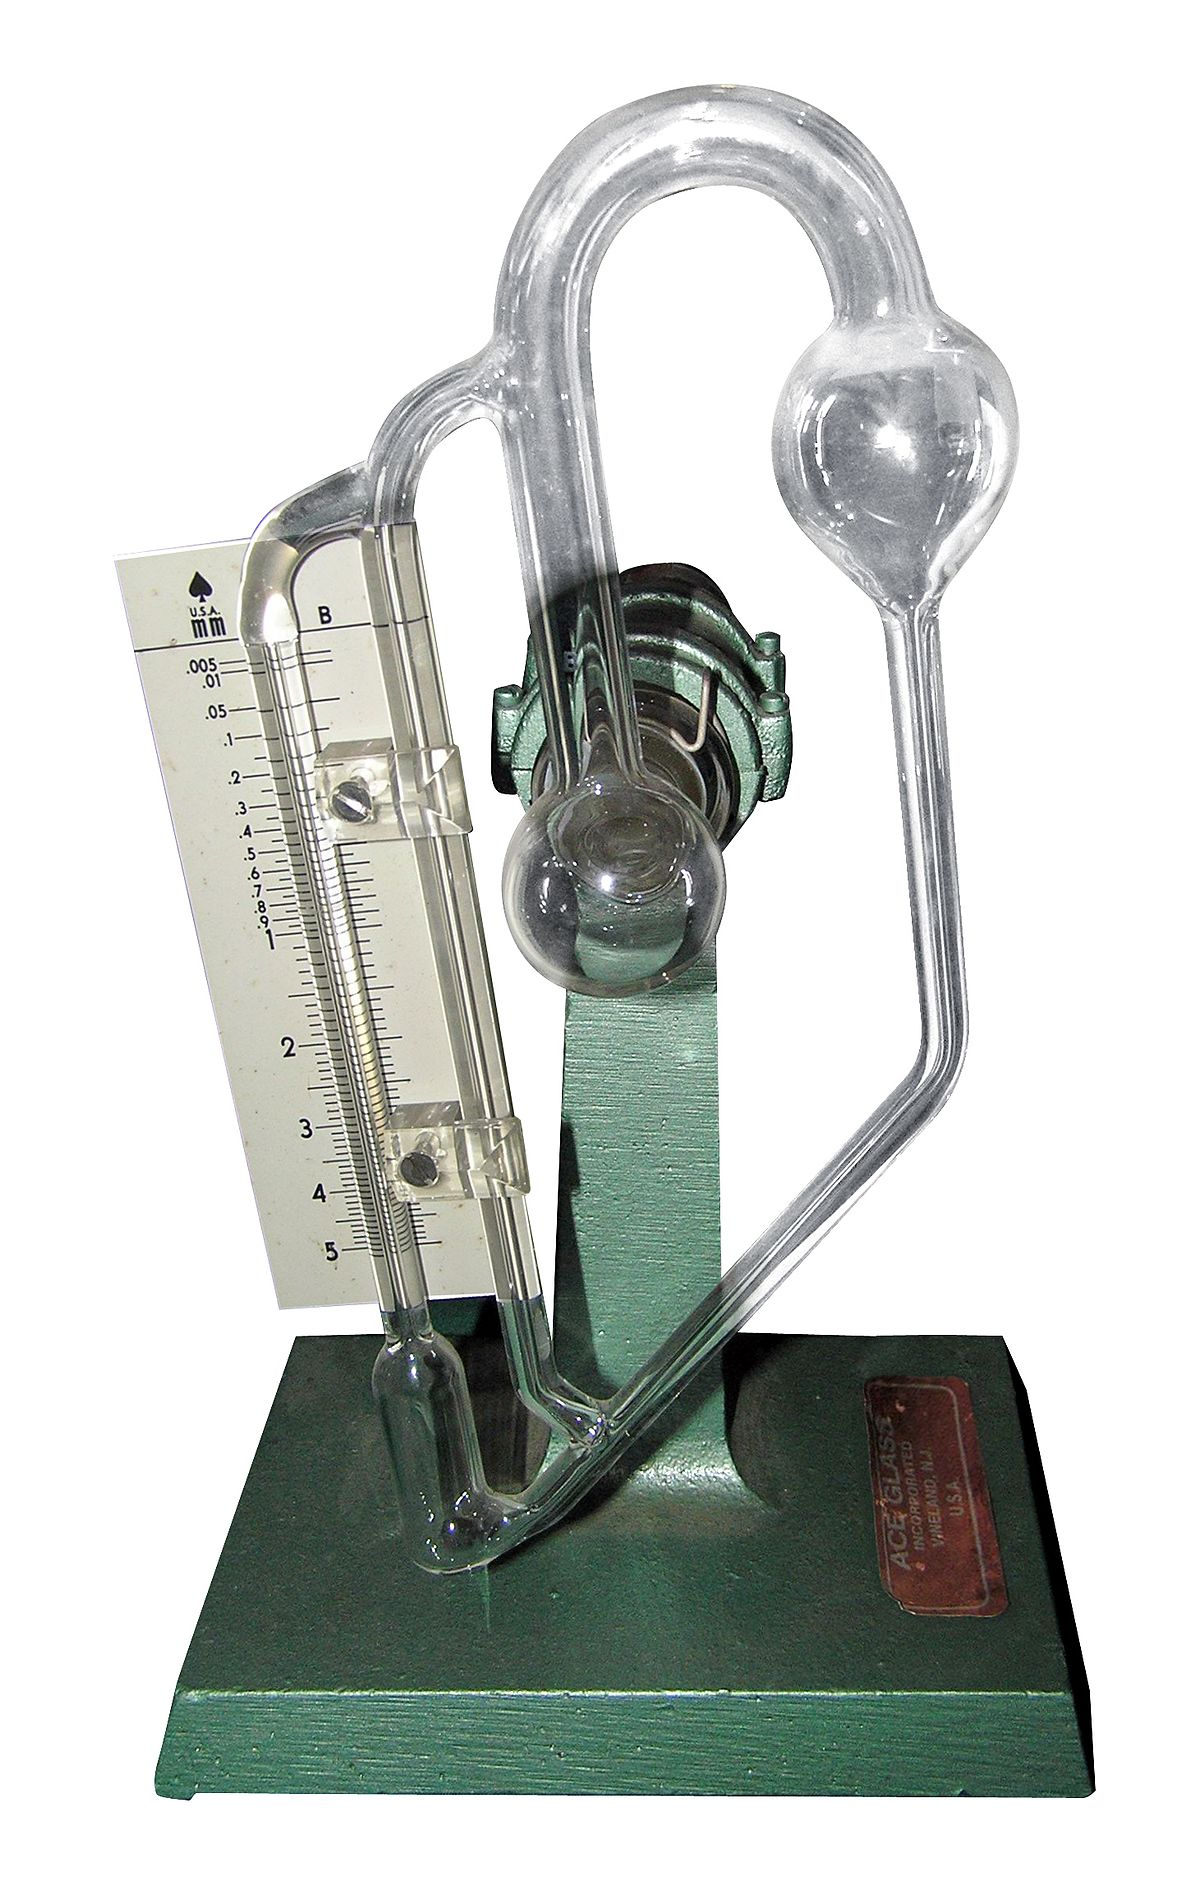
\includegraphics[width=4cm]{fig/Presion/McLeod_gauge_01.jpg}
             \\ \tiny{\href{https://en.wikipedia.org/wiki/McLeod_gauge}{Medidor McLeod}}
        \end{column}
        \begin{column}{0.5\textwidth}
            \begin{itemize}
                \item Empleados en medidas de alto vacío. Con lo cual resultan muy sensibles, costosos y complejos de calibración 
                \item Existen varios tipos:
             \begin{itemize}
                 \item Medidor McLeod.
                 \item Mecánicos – Tubo Bourdon, fuelle y diafragma.
                 \item Propiedades de un gas – Conductividad térmica.
                 \item Térmicos – Termopar, Pirani, bimetal.
                 \item Ionización – Filamento caliente, cátodo frío.
             \end{itemize}
            \end{itemize}
        \end{column}
    \end{columns}
\end{frame}

\begin{frame}{Campos de trabajo. Elementos Electrónicos de Vacío}
            \centering
            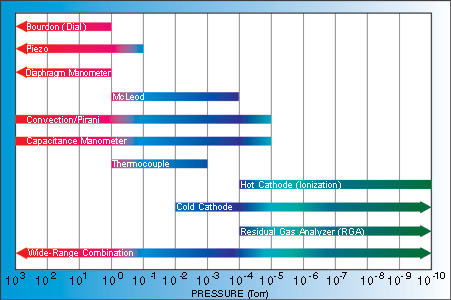
\includegraphics[width=9.5cm]{fig/Presion/Vaccuum Gauges.jpg}
             \\ \tiny{\href{https://www.lesker.com/newweb/technical_info/vacuumtech/pressure_04_bestgauge.cfm}{Campo de trabajo por tecnología}}
       
\end{frame}


\begin{frame}{Elementos electrónicos de vacío}
 \begin{table}[]
 \footnotesize
    \centering
    \begin{tabular}{m{3.2cm} m{1.2cm} m{1.2cm} m{1.9cm} m{1.8cm} m{1.6cm}}
        \toprule
        \textbf{Tipo de Sensor} & \textbf{Margen [torrs]} & \textbf{Escala} &\textbf{Exactitud}\\
        \midrule
        \textbf{Mecánicos} & 760-5 & Lineal & 1 \% \\
        \textbf{McLeod} & $5 - 10^{-3}$ & Lineal & 1-10 \% \\
        \textbf{Termopar} & $0.5 - 10^{-3}$ & Logarítmica & Alta\\
        \textbf{Pirani} & $2 - 10^{-3}$ & Logarítmica & -- \\
        \textbf{Bimetal} & $1 - 10^{-3}$ & Logarítmica & -- \\
        \textbf{Filamento Caliente} & $10^{-3} - 10^{-13}$ & Logarítmica & 1-10 \% \\
        \textbf{Cátodo frío} & $10^{-2} - 10^{-7}$ & Logarítmica & 1-10 \% \\
        \bottomrule
    \end{tabular}
    \caption{Comparación entre distintos tipos de presión electrónicos de vacío} \cite{sole2005instrumentacion}
    \label{tab:Comparacionvacio}
\end{table}
\end{frame}


\begin{frame}{Referencias}
\bibliographystyle{ieeetr}
\footnotesize
\bibliography{comunes/referencias}
\end{frame}

\end{document}